\documentclass[oupdraft]{bio}
\usepackage{url}

\usepackage{amsmath}
\usepackage{xparse}
\usepackage{mathtools}
\usepackage[table,dvipsnames]{xcolor}


\usepackage{ifthen}
\usepackage{pstricks}
\usepackage[normalem]{ulem}

\DeclareMathOperator*{\argmin}{arg\,min}
\DeclareMathOperator*{\argmax}{arg\,max}

\newcommand{\kmax}{k_{\text{max}}}
\newcommand{\lambdagrid}{\lambda^{\text{grid}}}



\newboolean{DEBUG}
\setboolean{DEBUG}{true}

\newrgbcolor{amycolor}{.7 .1 .1}
\ifthenelse {\boolean{DEBUG}}
{\newcommand{\amy}[1]{{\bf \amycolor{[\@Amy: #1]}}}}
{\newcommand{\amy}[1]{}}

\newrgbcolor{alexcolor}{.1 .7 .7}
\ifthenelse {\boolean{DEBUG}}
{\newcommand{\alex}[1]{{\bf \alexcolor{[\@Alex: #1]}}}}
{\newcommand{\alex}[1]{}}

\newrgbcolor{editcolor}{.1 .5 .7}
\ifthenelse {\boolean{DEBUG}}
{\newcommand{\edit}[1]{{\bf \editcolor{[\@edit: #1]}}}}
{\newcommand{\edit}[1]{}}

\begin{document}


% Title of paper
\title{Tuning parameter selection for a penalized estimator of species richness}

% List of authors, with corresponding author marked by asterisk
\author{ALEX PAYNTER, AMY D WILLIS$^\ast$\\[4pt]
% Author addresses
\textit{Department of Biostatistics,
University of Washington,
Health Sciences Building, Box 357232,
1705 NE Pacific St., Seattle, WA 98195}
% \\[2pt]
% % E-mail address for correspondence
% {payntera@uw.edu, adwillis@uw.edu}
}

% Running headers of paper:
\markboth%
% First field is the short list of authors
{A. Paynter and A.D. Willis}
% Second field is the short title of the paper
{Tuning parameter selection for species richness}

\maketitle

% Add a footnote for the corresponding author if one has been
% identified in the author list
\footnotetext{adwillis@uw.edu}

\begin{abstract}
{Our goal is to estimate the true number of classes in a population, called the species richness.  We consider the case where multiple frequency count tables have been collected from a homogeneous population, and investigate a penalized maximum likelihood estimator under a negative binomial model.
Our method penalises the probability of a class being unobserved, since high probabilities of unobserved classes increase the variance of species richness estimates. Tuning the penalisation parameter is challenging because the true species richness is never known, and so we propose and validate four novel methods to tune the penalization parameter.  We illustrate the performance of the method by estimating the microbial diversity of Lake Champlain over ...}
\end{abstract}

% TODO(Amy)
% - go through all references and confirm used correctly

\section{Introduction}
\label{sec:introduction}

The \textit{species problem} concerns estimating the number of classes $C$ that are present in a population.
$n$ individuals from the population can be sampled to find which classes they belong to, but since the  number of individuals in the sample is less than the total population size (which may be infinite), only $c$ classes are observed ($c \leq C$). The problem is named for its origins in biological ecosystems, where $C$ is \textit{species richness}, or the total number of species.  However, methods developed for the species problem can be applied to applications far removed from biology.  For example, \citet{efron_1976} estimated the number of words Shakespeare truly knew by modeling the frequencies of words in his published work, and  \citet{fegatelli_2018} estimated the number of cars covered by an insurer based on accident data where $c$ cars had at least one accident.

In ecology, species richness is a quantitative measurement of ecosystem diversity.  We focus on the specific application of estimating microbial diversity, that is, the number of strains of bacteria present in a population (e.g., a lake microenvironment or in an individual's oral cavity).
Microbial diversity is often linked with ecosystem health, such as in the vaginal microbiome (where high diversity is associated with infection \citep{Oakley:2008uo}) and in the gut microbiome (where high diversity is associated with healthy metabolism \citep{Morgan:2012bm,Minot:2019hc}).
Microbial abundance data typically contain many species observed infrequently (\textit{rare species}) and some which are observed a large number of times (\textit{abundant species}).  In data with both many rare and many abundant species, richness estimation methods often have high variance \citep{wang_2005,willis_2015}, motivating our regularised approach to estimation.

In this paper we consider the penalized maximum likelihood approach of \citet{wang_2005} and investigate the open problem of selecting the penalization parameter. Because the true species richness $C$ is never observed for any sample, common approaches to tuning parameter selection (e.g., cross-validation) cannot be employed. We propose using biological replicates to aid tuning. %, and so we extend the proposal of \citet{wang_2005} to the analysis of independent but homogeneous ecosystems.
We find that replicate data is advantageous for tuning the required penalization parameter and provide a comparison of the performance of 4 proposed methods for tuning parameter selection.

This paper is organized as follows: We review species richness estimation in Section \ref{sec:literature_review}.  In Section \ref{sec:fixed_lambda} we describe our extension to biological replicates, and in Section \ref{sec:efficacy_sims} we establish the utility of penalization via simulations. In Section \ref{sec:tuning_proposals} we propose several novel methods for tuning the penalization parameter, and in Section \ref{sec:tuning_simulations}
we evaluate our proposals. \amy{Section \ref{sec:data_analysis} applies our methods to microbiome data on Lake Champlain...} Section \ref{sec:discussion} closes with an expanded discussion of our results and suggested directions for future work. Software implementing the methods is available in the \url{R} package \url{rre}, available at \url{github.com/statdivlab/rre}, and code to reproduce the simulation results is available at \url{github.com/statdivlab/rre_sims}.


\section{Literature Review}

\label{sec:literature_review}

\subsection{Poisson mixture models}

The classical model for estimating species abundance is a Poisson mixture model.  Under this model the number of times we observe an species $i$ is $X_i \sim \text{Poisson}(\Lambda)$ where $\Lambda$ is a random variable distributed according to some mixing distribution.
Many mixing distributions have been proposed, including by  \cite{bulmer_1974,ord_1986,norris_1998} (see \cite{bunge_1993} for a comprehensive review). While our proposal may be easily generalized to other mixing distributions, in this paper we consider the Gamma  distribution for $\Lambda$, first considered by \citet{fisher_1943}.


Let $f_k = \#\{i: X_i = k\}$ be the number of classes observed $k$ times, called the \textit{frequencies} or \textit{frequency counts}.  Then the set $\{f_k\}_{k \geq 1}$ is a \textit{frequency count table}, a common way to represent species abundance data. Because $C = f_0 + f_1 + f_2 + \dots = f_0 + c$, the species problem can be framed as predicting $f_0$ to obtain the species richness estimate $\hat{C} = \hat{f}_0 + c$.

Let $\Lambda \sim \text{Gamma}(\alpha, \delta)$ with distribution function $f(\lambda) = \delta^\alpha \Gamma (\alpha)^{-1} \lambda^{\alpha - 1} e^{-\delta \lambda}$, and write $\eta = (\alpha, \delta)$.
% Then the distribution of $X_i$ under a gamma-Poisson model can written as a negative-binomial distribution,
% \begin{align}
% p_{\eta}(x) = \frac{\Gamma (x + \alpha)}{\Gamma (\alpha) x!} \left(\frac{\delta}{1+\delta} \right)^\alpha \left( \frac{1}{1+ \delta} \right)^x.
% \end{align}
% Note that we are interested in estimating the parameters of a negative binomial
% a zero-truncated negative binomial
%
There exist both frequentist \citep{fisher_1943} and Bayesian \citep{efron_1976,barger_2010} approaches to parameter estimation under this model. We will focus on frequentist maximum likelihood in this paper.
\amy{introduce Gamma later?}

\subsection{Estimation and computation}

The most straightforward maximum likelihood approach is to simultaneously maximize $C$ and $\eta$ using the full likelihood, which is known as the \textit{direct} approach.  A complication is that we have continuous parameters $\eta$ as well as one discrete parameter $C$, and so derivative-based optimization methods are not appropriate.  This issue has been studied by \citet{lindsay_1987}, who provide a discrete analog to the score function for this model.  %However, they point out that the asymptotics required use $C \to \infty$, which may not be appropriate for all problems.
Two other approaches to likelihood maximization are the \textit{conditional} and \textit{profile} approaches.  The conditional approach \citep{sanathanan_1977} involves writing the likelihood as the product
\begin{align}
 L(C, \eta) &= L_b(C, \eta)L_c(\eta) \label{eq:likelihood}
\end{align}
where
 \begin{align}
 L_b(C, \eta) &= \frac{C!}{(C-c)! \ c!} \left[1 - p_{\eta}(0) \right]^c \left[ p_{\eta}(0) \right]^{C-c}  %& \text{(``Binomial'' component)}
  \label{eq:binomial_likelihood}\\
 L_c(\eta) &= \frac{c!}{\displaystyle  \prod_{k \geq 1} f_k!} \prod_{k \geq 1} \left[ \frac{p_{\eta}(k)}{1-p_{\eta}(0)} \right]^{f_k}. \label{eq:conditional_likelihood} % & \text{(Multinomial component/``conditional'')}
\end{align}
We see that the likelihood is the product of a binomial probability mass function $c \sim$ Binomial $\left(C, 1- p_{\eta}(0)\right)$, and a multinomial probability mass function $(f_1, f_2, \ldots)|c \sim$  Multinomial $\left(c,  \frac{(p_{\eta}(1), p_{\eta}(2), \ldots)}{1-p_{\eta}(0)}\right)$.
This decomposition is convenient because $L_c$ is a function of $\eta$ alone.
% $L_b$ shows the probability of observing $c$ species follows a binomial distribution, i.e. $c \sim \text{Binomial}\left(C, 1- p_{\eta}(0)\right)$.  Letting $\kmax$ be the largest $k$ such that $f_k > 0$, $L_c$ shows that observing the frequency counts given by $f_1, f_2, \dots , f_{\kmax}$ follows a multinomial distribution given $c$.  The multinomial cell probabilities are proportional to $p_{\eta}(k)$.
\citet{sanathanan_1977}'s conditional approach to optimization involves first maximising  $L_c(\eta)$ to obtain a conditional abundance estimate $\widehat{\eta}_c$, then maximising $L_b(C, \widehat{\eta}_c)$ over $C$.
The conditional estimate of $C$ is then
\begin{equation}
\widehat{C}_c = \Biggl\lfloor \frac{c}{1-p_{\widehat{\eta}_c}(0)} \Biggr\rfloor \label{eq:conditional_c}
\end{equation}
where $\lfloor a \rfloor$ is the largest integer less than or equal to $a$.  In the \textit{profile} likelihood approach the expression in Equation \eqref{eq:conditional_c} is substituted into the full likelihood, which gives us a function of $\eta$ alone (see \citet{wang_2005}).  The conditional and profile approaches have been shown to be asymptotically equivalent to the direct approach.
\amy{Need to justify why we are bringing this up}

% \citet{sanathanan_1977} uses this decomposition to propose the conditional approach to likelihood maximization, which is done in two steps (see \citet{chao_2002} for a detailed presentation).  First we maximize $L_c(\eta)$ to obtain a conditional abundance estimate $\widehat{\eta}_c$.  Then $L_b(C, \widehat{\eta}_c)$ is maximized over $C$.  With $\eta$ fixed there is a closed form expression for this second step,
% \begin{equation}
% \widehat{C}_c = \Biggl\lfloor \frac{c}{1-p_{\widehat{\eta}_c}(0)} \Biggr\rfloor %\label{eq:conditional_c}
% \end{equation}
% where $\lfloor a \rfloor$ is the largest integer less than or equal to $a$.  In the \textit{profile} likelihood approach the expression in Equation \eqref{eq:conditional_c} is substituted into the full likelihood, which gives us a function of $\eta$ alone (see \citet{wang_2005}).  The conditional and profile approaches have been shown to be asymptotically equivalent to the direct approach.

\subsection{Challenges with Poisson mixture models}


A perennial issue in the species problem, especially for microbial datasets, is the instability of species richness estimators \citep{Rocchetti:2011tv,willis_2015}.
%
% Under the gamma-Poisson model,
%
% To illustrate, consider that a first-order approximation gives $$Var(\hat{C}_c | c) \approx \frac{c^2}{(1-\hat{p}(0))^4}Var(\hat{p}(0))$$ \amy{check this}
% Therefore,
% , especially maximum likelihood estimators.  The estimates often have unacceptably high variance and can become dramatically inflated.
%
%\sout{\textcolor{blue}{Since $Pr(X = 0) = \left( \frac{\delta}{1 + \delta}\right)^\alpha$, if there are many low abundance species then $\alpha$ will be near 0. Many high abundance species, as we see in microbial data, tends to cause $\delta$ to be near 0 as well.  The tendency of both abundance parameters to be near their boundary is one way to explain why this instability issue has plagued the species problem over a variety of approaches, and is especially prominent in microbial data.}}
%% One way of improving stability is to abandon the Poisson mixture paradigm entirely.  Though we will focus on the gamma-Poisson model in this paper, we would be remiss if we did not briefly mention other popular alternatives.  Coverage-based estimators, which use the proportion of species observed $k$ times rather than the actual counts were originally proposed by \citet{good_1953} and remain popular.  Capture-recapture methods (see \citet{chao_1987}) have a deep literature in animal abundance studies but are not as applicable in microbial data where the sampling  destroys the organism.  See \citet{bunge_1993} for a comprehensive review and \citet{bunge_2014} for an updated review of species richness methods which are outside the scope of this paper.
A proposal which encourages stability of estimates under Poisson-mixture models is due to \citet{wang_2005}.  Their proposal is to add a penalty term to the log likelihood that penalizes the probability of observing a species zero times. They consider the
penalized log likelihood
\begin{equation}
\ell_\lambda(C, \eta) = \ell(C,\eta) - \lambda \log p_{\eta}(0)
\label{eq:wang_lindsay}
\end{equation}
where $\ell(C,\eta) = \log L(C, \eta)$ is the log likelihood and $\lambda > 0$ is a penalization parameter.
Let $\hat{C}_\lambda = \arg \max_{C} \ell_\lambda(C, \eta)$.
Then, for $\lambda \geq \lambda',$ $\hat{C}_\lambda \leq \hat{C}_{\lambda'}$ \citep[Theorem 1]{wang_2005}. In particular, for $\lambda > 0,$ the penalized maximum likelihood solution $\hat{C}_\lambda$ is less than or equal to $\hat{C}_0$, the maximum likelihood estimate. Furthermore, for a large enough $\lambda$, $\hat{C}_\lambda = c$; that is, the penalised maximum likelihood estimate shrinks to the observed richness $c$.
\citet{wang_2005} also consider two other penalty functions of similar form, which we do not discuss here except to note that our tuning parameter selection methods would equally apply.


\citet{wang_2005} show that a trade-off exists: greater values of $\lambda$ correspond to a more stable estimator, but at the potential cost of negative bias.
The choice of penalization parameter implies a preference for lower variance or lower bias, adding subjectivity to the estimation procedure.
\citet{wang_2005} note that a limitation of their proposal is that ``one must select a penalty function and a tuning parameter, and it is nigh impossible to make convincing statements about why one choice should be uniformly superior to another.''
Furthermore, we expect different data sets to require different $\lambda$ values for optimal mean squared error.
% Our primary interest in studying the analysis of replicate frequency count tables is to leverage the replicates to tune the penalization parameter in Equation \eqref{eq:wang_lindsay}.
The goal of this paper is to propose and investigate data-adaptive methods to select $\lambda$.


\section{Extension to Replicate Data}
\label{sec:fixed_lambda}

We focus on the gamma-Poisson model and penalised log-likelihood of the form \eqref{eq:wang_lindsay}, and consider the case where we observe $r$ independent frequency count tables from the population under study.
% with penalization as proposed by \citet{wang_2005}.  In this section we extend the penalized likelihood for a single frequency count table to the case where multiple frequency count tables have been collected.
We will assume that these $r$ frequency count tables are biological replicates drawn independently from the same population, i.e. they have a common structure specified by the parameters $C$ and $\eta$.  A set of $r$ frequency count tables from the same population will be called a \textit{sample}, and a single frequency count table will be referred to as a \textit{replicate}.  Let the number of species observed $k$ times in replicate $j$ be $f_{kj}$, $j \in \{1, \dots , r\}$.  Let $c_j$ be the observed richness in replicate $j$.

% Microbial data is often available as labeled abundance information $\{ X_{ij} \}$, the number of times species $i$ was observed in replicate $j$.  In this paper we study data represented in frequency counts $\{f_{kj}\}$ and it is worth pointing out that we lose some information in this representation.  For instance, in sample of frequency count tables it cannot be determined whether species $i$ was observed in two different replicates.  By using a mixed Poisson model we assume a common abundance structure between the species in order to estimate $C$.  While there may be other methods which leverage the additional information in an abundance table representation, the frequency counts are a minimal sufficient statistic for mixed Poisson models.

In Section \ref{sec:tuning_proposals} we will require an objective function defined in terms of a subset of indices of the frequency count tables, so we define it that way now.  Let $J \subseteq \{1, \dots, r\}$.  $J$ indicates the data being used in the evaluation of the objective function, with $J = \{1, \dots r\}$ meaning we use all replicates.  Let $\ell \left(C, \eta; \{f_{kj}\}_{k \geq 1} \right)$ be the unpenalized log likelihood for replicate $j$.
Using the fact that the draws are independent, our objective function for a fixed $\lambda \geq 0$ is the sum of the log likelihoods for each individual replicate.
We define the \textit{penalized log likelihood} for multiple samples as
\begin{align}
\mathcal{O}_{\lambda}(C, \eta; J) :=& \sum_{j \in J} \ell \left(C, \eta; \{f_{kj}\}_{k \geq 1} \right) - \lambda\log p_{\eta}(0) \\
 =& \sum_{j \in J} \biggl[ \log C! - \log (C-c)! + (C-c) \log p_\eta(0)  \nonumber \\
 & \qquad  - \sum_{k \geq 1} \log{} f_{kj}! + \sum_{k \geq 1} f_{kj} \log p_\eta(k) \biggr] - \lambda \log p_\eta(0)    \label{eq:objective}
\end{align}
By fixing $\lambda = 0$ we obtain the \textit{unpenalized log likelihood} for all replicates $j \in J$.  We define $\widehat{C}_{\lambda}$ to be the penalized maximum likelihood estimate for based on tuning parameter $\lambda$, that is,
\begin{equation}
\left(\widehat{C}_{\lambda},  \widehat{\eta}_{\lambda} \right) = \argmax_{C, \, \eta}  \mathcal{O}_{\lambda} \left(C, \eta ; \{1, \dots , r\} \right) \label{eq:ccc_hat_lambda}
\end{equation}
where $\widehat{\eta}_{\lambda}$ is a nuisance parameter.

We use root-mean-square error as the primary criterion for evaluating the performance of estimators in simulations.  Let $n_{\text{sim}}$ be the number of simulations completed for one choice of $(C, \eta, r)$, and $\widehat{C}_{\lambda \langle s \rangle}$ be the solution of Equation \eqref{eq:ccc_hat_lambda} obtained in simulation number $s$ with  $\lambda$.  Then we define
\begin{equation}
 \text{RMSE}\left( \widehat{C}_{\lambda} \right) = \sqrt{ \frac{1}{n_{\text{sim}}} \sum_{s=1}^{n_{\text{sim}}} \left( \widehat{C}_{\lambda \langle s \rangle} - C\right)^2 }
\end{equation}

To maximize the likelihood we will use the direct approach, rather than the profile and conditional approaches reviewed in Section \ref{sec:literature_review}.  While it may be faster to use the profile or conditional approach, our investigations revealed that the results are not always the same in finite samples.
Since our objective is to evaluate approaches to tuning, we place priority on the accuracy of optimization over speed.

To implement a direct optimization approach we search over candidate $C$ values in a grid.  A gradient-based search over $\eta$ values is used at each $C$ in the grid to find the maximum penalised likelihood  $(C, \eta)$.

\section{Efficacy of Penalization}
\label{sec:efficacy_sims}
\subsection{Simulation setup}

Before evaluating potential tuning parameter selection methods, we first establish that penalization can improve richness estimation.  \citet{wang_2005} established that it can improve estimates for $r = 1$, this needs to be verified for $r> 1$.
We propose simulating data under the gamma-Poisson model and maximizing the objective function with a set of fixed $\lambda$ values.  If there exists some $\lambda > 0$ where RMSE($\widehat{C}_{\lambda}$) is less than RMSE($\widehat{C}_0)$, we conclude that penalization is effective for the given data generating mechanism.

We simulated using $C = 1000$, and $r \in \{6, 10, 14\}$.  We found that $\eta = (\alpha, \delta) = (10^{-1}, 10^{-1})$  provided a good fit to the data of  \citet{walsh2014restricted}, and $\eta = (10^{-2}, 10^{-5})$ provided a good fit to the data of \citet{tromas_2017}.
For completeness we also investigated nearby $\eta$ values: $\eta = \left( 10^{-1}, 10^{-3} \right)$ and $\eta = \left( 10^{-1}, 10^{-5}\right)$.
% To select $\eta$, we investigated the unregularised
%  two microbial datasets
% so choosing appropriate simulation values of $\eta$ is crucial in targeting our approach to microbial data.   We used two microbial datasets as motivating examples.  \citet{walsh2014restricted} provide a dataset from soil in a Swiss apple orchard and we found $\eta = (\alpha, \delta) = (10^{-1}, 10^{-1})$ produced a frequency count table with a similar structure to their data.  The second example from \citet{tromas_2017} is a sample of cyanobacteria from Lake Champlain, and we found $\eta = (10^{-2}, 10^{-5})$ mimicked the structure of their data well.  We note that is possible that the gamma-Poisson model is not the best fit for these examples, but our goal is only to choose $\eta$ in an appropriate range.  Two nearby $\eta$ values are included, $\eta = \left( 10^{-1}, 10^{-3} \right)$ and $\eta = \left( 10^{-1}, 10^{-5}\right)$.  These add variety to our simulations in this section and context for our simulations in Section \ref{sec:tuning_simulation_2}.  Under each combination of $\eta$ and $r$ 100 simulations were completed.
In Table \ref{tab:eta_intuition} we provide a few summary measures for frequency count tables generated under each choice of $\eta$.  This characterizes the $\eta$ values by the proportion of unobserved, rare or abundant species we would expect to see. We return to a discussion of the different data structures in Section \ref{sec:tuning_simulations}.
For each combination of $\eta$ and $r$, we performed 100 simulations.
We investigated the grid $\lambda \in \{0, 5, \dots , 120\}$, and found that this grid was sufficiently expansive to ensure that the RMSE-minimising $\lambda$ was not on the boundary of the grid
(see Figures \ref{fig:fixed_lambda} and \ref{fig:fixed_lambda_2}).


% One final setting is necessary for these simulations: a set of $\lambda$ values to test over.  Our primary concern is to ensure the set covers the optimal value, i.e. $\lambda$ which produces the lowest RMSE$(\widehat{C}_{\lambda})$.  While we do not have a theoretical way to determine the ideal $\lambda$ set, we can use the known behavior of the penalty function to confirm that the set was sufficiently large after the simulation is complete.  As $\lambda$ increases, $\widehat{C}_{\lambda}$ decreases.  If $\widehat{C}_{\lambda_0}$ is  below the true $C$, then for $\lambda > \lambda_0$ $\widehat{C}_{\lambda}$ will be further from $C$, and the RMSE will increase.  Then we can be assured that the set is large enough if most or all simulations had a $\widehat{C}_{\lambda}$ below the truth for the largest $\lambda$ tested.
% This is clearly verifiable in the cases presented in Figures \ref{fig:fixed_lambda} and \ref{fig:fixed_lambda_2}. Simulating using $\lambda \in \{0, 5, \dots , 120\}$ was sufficient for all simulations in this section.


% latex table generated in R 3.5.1 by xtable 1.8-2 package
% Thu May 23 22:11:47 2019
\begin{table}[t]
\tblcaption{The expected proportion of unobserved ($k=0$), singleton ($k=1$), rare ($k=1,2,3$), and abundant  ($k \geq 10$) species for 4 choices of $\eta$.  We also give the expected frequency count of the most abundant species when $C = 1000$.
\label{tab:eta_intuition}}
\centering
\footnotesize
\begin{tabular}{rcccc}
  \hline
 $\eta = $ & ($10^{-1}$, $10^{-1}$) & ($10^{-2}$, $10^{-5}$) & ($10^{-1}$, $10^{-3}$) & ($10^{-1}$, $10^{-5}$) \\
  \hline
  Proportion unobserved ($p_{\eta}(0)$) & 0.787 & 0.891 & 0.501 & 0.316 \\
  Proportion singletons ($p_{\eta}(1)$) & 0.072 & 0.009 & 0.050 & 0.032 \\
  Proportion rare ($\sum_{k=1}^3 p_{\eta}(k)$) & 0.130 & 0.016 & 0.097 & 0.061 \\
  Proportion abundant ($\sum_{k=10}^{\infty} p_{\eta}(k)$) & 0.028 & 0.083 & 0.340 & 0.583 \\
Expected max abundance ($\mathbb{E}\left[k_{\text{max}}\right]$) & $4.1 \times 10^{1}$ & $2.0 \times 10^{5}$ & $4.0 \times 10^{3}$ & $3.9 \times 10^{5}$ \\
   \hline
\end{tabular}
\normalsize
\end{table}



\begin{table}[h]
\tblcaption{The penalised maximum likelihood estimate of $C$ has lower RMSE for all investigated choices of $\eta$ and $r$ under a Gamma-mixed Poisson model for species abundances based on 100 simulations for each choice of $\eta$ and $r$.
$\lambda_{\text{opt}}$ is the value of $\lambda$ which produced the lowest RMSE.
$\widehat{C}_0$ is the $C$ estimate with $\lambda = 0$, and $\widehat{C}_{\lambda_{\text{opt}}}$ is the $C$ estimate using $\lambda = \lambda_{\text{opt}}$.
\label{tab:fixed_lambda_results}}
\centering
\begin{tabular}{ccccc}
  \hline
$\eta = (\alpha, \delta)$ & $r$ & RMSE ($\widehat{C}_{0}$) & $\lambda_{opt}$ & RMSE ($\widehat{C}_{\lambda_{ \text{opt}}}$) \\
  \hline
$\left(10^{-1}, 10^{-1}\right)$ &   6 & 796.90 &  10 & 326.50 \\
$\left(10^{-1}, 10^{-1}\right)$ &  10 & 527.53 &  15 & 286.27 \\
  $\left(10^{-1}, 10^{-1}\right)$ &  14 & 337.31 &  10 & 235.51 \\
  $\left(10^{-2}, 10^{-5}\right)$ &   6 & 735.95 &  15 & 516.37 \\
  $\left(10^{-2}, 10^{-5}\right)$ &  10 & 700.21 &  20 & 456.04 \\
  $\left(10^{-2}, 10^{-5}\right)$ &  14 & 666.55 &  20 & 470.35 \\
  $\left(10^{-1}, 10^{-3}\right)$ &   6 & 200.09 &  20 & 156.29 \\
  $\left(10^{-1}, 10^{-3}\right)$ &  10 & 213.22 &  55 & 142.64 \\
  $\left(10^{-1}, 10^{-3}\right)$ &  14 & 243.42 &  55 & 148.26 \\
  $\left(10^{-1}, 10^{-5}\right)$ &   6 & 401.17 &  55 & 147.13 \\
  $\left(10^{-1}, 10^{-5}\right)$ &  10 & 283.91 &  25 & 137.04 \\
  $\left(10^{-1}, 10^{-5}\right)$ &  14 & 415.19 &  70 & 126.72 \\
   \hline
\end{tabular}
\end{table}

\subsection{Simulation results} \label{sec:first_sim}

The results of the simulation are shown in Table \ref{tab:fixed_lambda_results}.  For every parameter choice a reduction in RMSE($\widehat{C}_{\lambda}$) is found for some $\lambda > 0$.  Depending on simulation parameters the reduction varied from 22\% to 70\% compared to RMSE($\widehat{C}_{0}$) for the best $\lambda$.  These results show that for a variety of $(\eta, r)$ choices, penalization improves species richness estimation.
We also see that the optimal $\lambda$ value varies considerably over $(\eta, r)$, ranging from 10 to 70.  This suggests that there is not a universally appropriate $\lambda$ choice. Therefore, tuning $\lambda$ to the sample appears desirable. We note that the optimal choice of $\lambda$ is not consistent either for fixed $r$ and variable $\eta$, nor for fixed $\eta$ and variable $r$.

In order to demonstrate the effect on $\widehat{C}_{\lambda}$ as we increase $\lambda$, we plot the results for two $\eta$ values in Figures \ref{fig:fixed_lambda} and \ref{fig:fixed_lambda_2}.  For small values of $\lambda$ we acquire lower variance in the estimates while incurring some negative bias, and the RMSE improves as a result.  Eventually the bias difference dominates and the RMSE increases as $\lambda \to \infty$.


\begin{figure}[p]
\caption{Simulation results for estimation of $C$ under a range of fixed $\lambda$ constants, $\eta = (10^{-1}, 10^{-1})$, over 100 simulations. The black line indicates the true value $C = 1000$.
\label{fig:fixed_lambda}}
\centering\makebox[\textwidth]{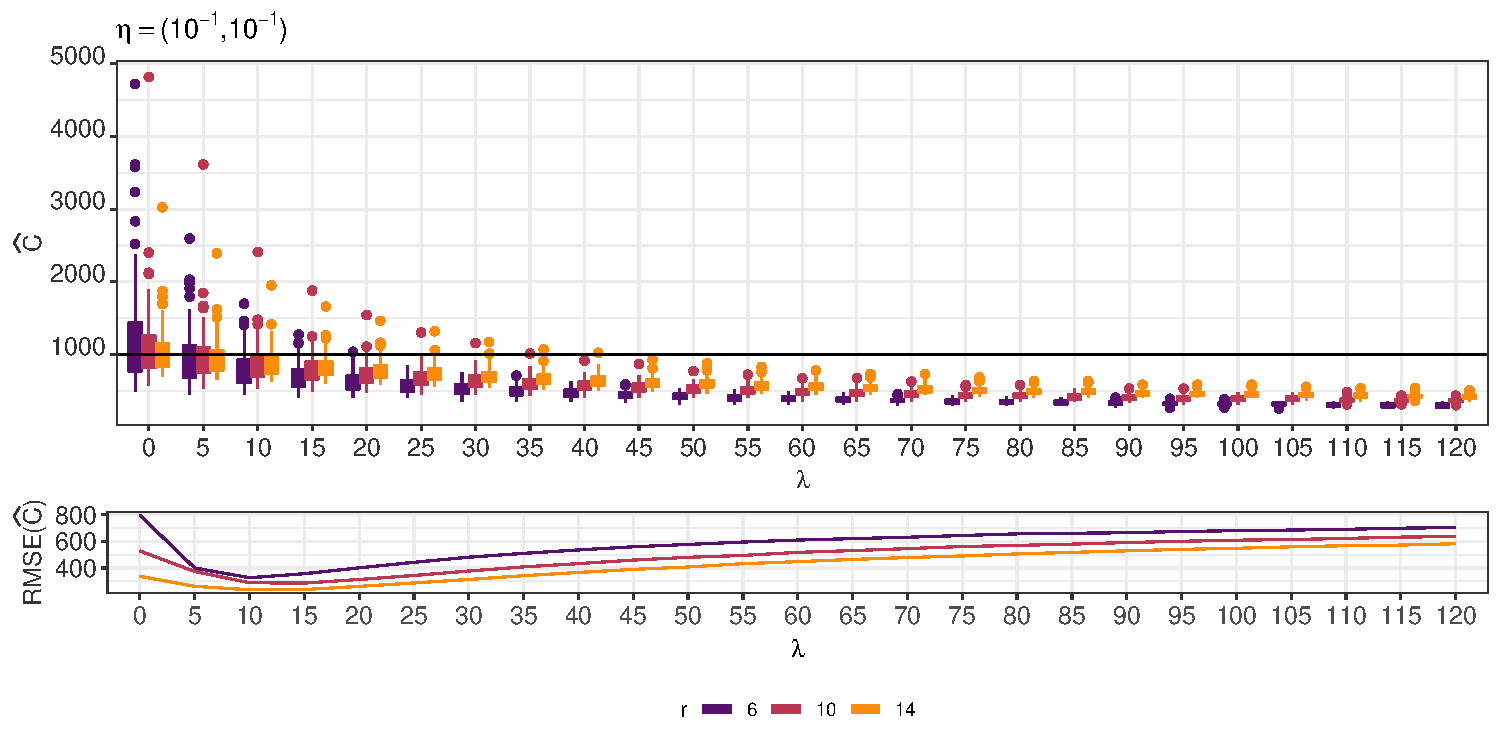
\includegraphics[width=1\textwidth]{./images/fixed_lambda_eta1.pdf}}
\end{figure}


\begin{figure}[p]
\caption{Simulation results for estimation of $C$ under a range of fixed $\lambda$ constants, $\eta = (10^{-2}, 10^{-5})$, over 100 simulations.  The black line indicates the true value $C = 1000$.
\label{fig:fixed_lambda_2}}
\centering\makebox[\textwidth]{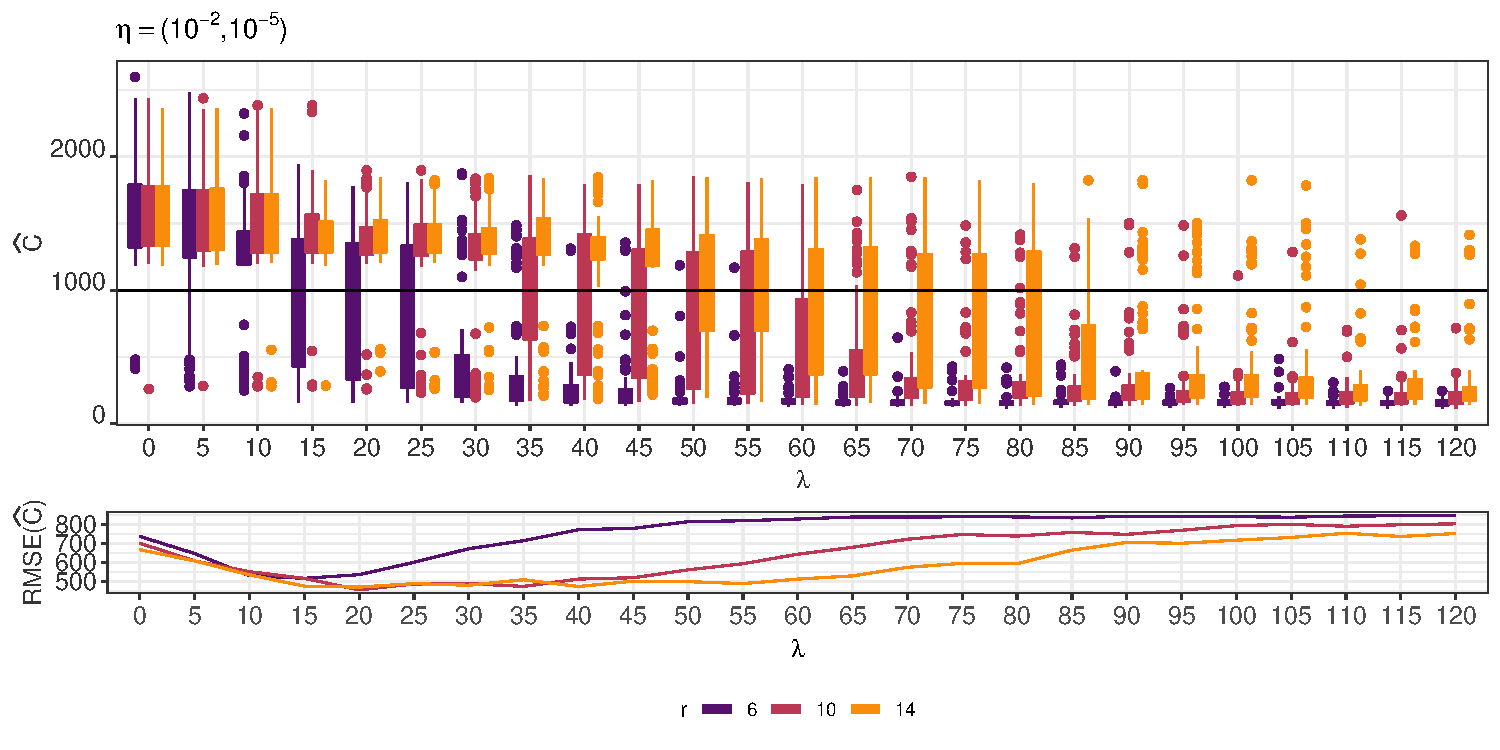
\includegraphics[width=1\textwidth]{./images/fixed_lambda_eta2.pdf}}
\end{figure}


%
%
%
\section{Methods for Tuning $\lambda$}
\label{sec:tuning_proposals}

We have established that penalization can improve richness estimates, but different abundance structures ($\eta$) require different penalization parameters ($\lambda$) to minimize RMSE.  Therefore a method which can tune the parameter based on a sample is warranted.  We propose several novel methods in this section.  Each is evaluated via simulation in Section \ref{sec:tuning_simulations}.

\setcounter{subsection}{-1}
\subsection{Method 0: MLE without penalization}

We compare all proposed methods to the unpenalised MLE using $J = \{1, \dots r \}$:
%Recall that fixing $\lambda = 0$ gives us the unpenalized likelihood in Equation \eqref{eq:objective}, and so by denoting the $C$ estimate obtained using Method 0 as $\widehat{C}_{[0]}$, then
\begin{equation}
\left(\widehat{C}_{[0]},  \widehat{\eta}_{[0]} \right) = \argmax_{C, \, \eta}  \mathcal{O}_{0}\left(C, \eta ; \{1, \dots , r\} \right) \label{eq:c_hat_0}
\end{equation}
This method is fast and simple, making it an ideal baseline for comparison

For all of the remaining methods (1-4) we generate estimates $\widehat{C}_\lambda$ over $\lambda \in \lambda^{\text{grid}}$, where $\lambdagrid$ is user-specified (e.g., $\lambdagrid = \{0, 5, 10, \dots 120\}$ in Section \ref{sec:first_sim}).  %The methods differ in how they subset the data to create these estimates, and in the steps they take to arrive at a final estimate $\widehat{C}_{\text{[method]}}$.

%
%
\subsection{Method 1: Minimum subset variance}

Ideally, our estimator for $C$ will have low variance, that is, there should be low variance in estimates from different resamples from the population.
% Method 1 is motivated by the belief that if we resample from the same population, an ideal $C$ estimator should have low variance.
Exploiting the fact that we have replicate data, we repeatedly partition the replicates into two subsets and calculate two estimates.  We then select the $\lambda$ which yields the lowest between-subset variance.  This partitioning is repeated $p$ times to average out the arbitrary choice of subsets.


Let $T_1(l)$ be the first subset of the $l^{\text{th}}$ partition and $T_2(l)$ be the second subset of the $l^{\text{th}}$ partition, for $l \in \{1, \dots , p\}$. That is, $T_i(l) \subseteq \{1, \dots , r\}$, $T_1(l) \cap T_2(l) = \emptyset$ and $T_1(l) \cup T_2(l) = \{1, \dots ,r\}$.
For each $\lambda \in \lambda^{\text{grid}}$, $l \in \{1, \dots, p\}$ let
\begin{align}
\left(\widehat{C}_{\lambda}^{ \ T_1(l)}, \widehat{\eta}_{\lambda}^{ \ T_1(l)} \right) &= \argmax_{C, \, \eta} \mathcal{O}_\lambda \left(C, \eta; T_1(l) \right) \\
\left(\widehat{C}_{\lambda}^{ \ T_2(l)}, \widehat{\eta}_{\lambda}^{ \ T_2(l)} \right) &= \argmax_{C, \, \eta} \mathcal{O}_\lambda \left(C, \eta; T_2(l) \right)
\end{align}
We now have a $\widehat{C}$ corresponding to each $\lambda \in \lambdagrid$ in each subset of each partition.  Our goal in Method 1 is to use these estimates to select the $\lambda$ value which gave us the lowest average variance over all partitions, denoted by $\widetilde{\lambda}_{[1]}$.  The overall estimate for Method 1, $\widehat{C}_{[1]}$, is a simple average of the estimates produced under $\widetilde{\lambda}_{[1]}$:
\begin{align}
\widetilde{\lambda}_{[1]} &= \argmin_{\lambda} \frac{1}{p} \sum_{l=1}^p \text{Var}\left[ \widehat{C}_{\lambda}^{ \ T_1(l)}, \widehat{C}_{\lambda}^{ \ T_2(l)} \right] \\
\widehat{C}_{[1]} &=  \frac{1}{p} \sum_{l=1}^p \left[ \frac{\widehat{C}_{\widetilde{\lambda}_{[1]}}^{ \ T_1(l)} + \widehat{C}_{\widetilde{\lambda}_{[1]}}^{ \ T_2(l)}}{2} \right]
\end{align}

In our simulations we chose an equal split of the indices for each partition: $|T_1(l)| = |T_2(l)|$.  The subsets of each partition are selected at random, so we could select the same subset split more than once.  We partition a total 10 times ($p = 10$).  For example, if $r = 4$ then $T_1(1) = \{1,4\}$ and $T_2(1) = \{2, 3\}$ would be a valid subset selection.  This holds in methods 2 and 4 as well, which also use partitioning.

\subsection{Method 2: Cross-validated likelihood}

\amy{up to here with editing}

A frequently employed method that takes advantage of replicate data is cross-validation.  Cross-validation is most commonly applied to evaluate the strength of a model in a dataset containing both features and outcomes.  The model is trained on one subset of the data and then evaluated using another.  However, in the species problem we never observe true outcomes, i.e. $C$ is always estimated using the frequency counts.  Methods 2 and 4 are motivated by the desire to do something similar to cross-validation, but we have to find a function which takes the place of mean prediction error in the absence of any true $C$ observations.

In Method 2 we use one subset of the data to generate estimates.  Then we evaluate those estimates using the likelihood with the data from the other subset.  As before, we partition the data into two subsets $p$ times, calling them $T(l)$ for the training subset of the $l$-th partition, and $E(l)$ for the evaluation subset of the $l$-th partition.  $T(l), E(l)$ are created exactly as in Method 1, we only relabel them to indicate the change in purpose.  Then for each $\lambda \in \lambdagrid$, $l \in \{1, \dots , p\}$ let
\begin{equation}
\left(\widehat{C}_{\lambda}^{ \ T(l)}, \widehat{\eta}_{\lambda}^{ \ T(l)} \right) = \argmax_{C, \, \eta} \mathcal{O}_\lambda \left(C, \eta; T(l) \right) \label{eq:part_c_hats_method_2}
\end{equation}
so that we have an estimate using only the training subset for each $\lambda$ value and each partition.  A $\lambda$ value is selected by plugging those estimates into the unpenalized likelihood with $J = E(l)$.
\begin{align}
\widetilde{\lambda}_{[2]} &= \argmax_\lambda \sum_{l=1}^p \mathcal{O}_0\left( \widehat{C}_{\lambda}^{ \ T(l)}, \widehat{\eta}_{\lambda}^{ \ T(l)} ; \  E(l) \right) \label{eq:selected_lambda_2} \\
\widehat{C}_{[2]} &= \frac{1}{p} \sum_{l=1}^p \widehat{C}_{\widetilde{\lambda}_{[2]}}^{ \ T(l)}
\end{align}
 In the evaluation step given in Equation \eqref{eq:selected_lambda_2} we must use the unpenalized likelihood, as opposed to the penalized version.  The penalty term is in fact always positive, and has the potential dominate the likelihood if a very large $\lambda$ exists in $\lambdagrid$. For example, suppose we used the penalized likelihood and $10^7 \in \lambdagrid$.  Then no matter what data was passed in, Method 2 would select $\widetilde{\lambda} = 10^7$, and $\widehat{C}_{[2]}$ would shrink to the observed richness as a consequence.

%
%
%
\subsection{Method 3: Goodness of fit}

We depart from our partitioning scheme to explore another desirable property of an estimator.  An ideal estimator would produce parameter estimates $\widehat{C}$, $\widehat{\eta}$ which fit well with the frequency counts in our sample.  Consider a single frequency count table.  Using Equation \eqref{eq:likelihood} we can find the expected frequency counts $f_k$ given $C$ and $\eta$,
\begin{equation}
 \mathbb{E}\left(f_k\right) = \mathbb{E}\left(f_k|c \right) = \mathbb{E}\left( c \frac{p_{\eta}(k)}{1-p_{\eta}(0)} \right) = C\left(1-p_{\eta}(0) \right) \frac{p_{\eta}(k)}{1-p_{\eta}(0)} = Cp_{\eta}(k)
\end{equation}
Then given estimates $\widehat{C}$ and $\widehat{\eta}$ we use a plug-in estimate for the expected counts: $\widehat{f_k} = \widehat{C}p_{\widehat{\eta}}(k)$.  If we consider each $f_k$ a category, the usual $\chi^2$ goodness of fit statistic is
\begin{align}
&\sum_{k=1}^{\infty} \frac{\left(f_k - \widehat{f}_k \right)^2 }{\widehat{f}_k} \\
&=\sum_{k=1}^{\infty} \frac{\left(f_k - \widehat{C}p_{\widehat{\eta}}(k) \right)^2 }{\widehat{C} p_{\widehat{\eta}(k)}}  \label{eq:chi_sq_compact} \\
& = \sum_{k=1}^{k_{max}} \frac{\left(f_k - \widehat{C}p_{\widehat{\eta}}(k) \right)^2 }{\widehat{C} p_{\widehat{\eta}(k)}} \ + \ \ \widehat{C} \sum_{k = k_{max}+1}^{\infty} p_{\widehat{\eta}}(k) \label{eq:chi_sq_expanded}
\end{align}
Equation \eqref{eq:chi_sq_expanded} uses the fact that we have some $k_{max}$ in every frequency count table such that $f_k = 0$ for all $k > \kmax$.  Therefore the statistic is a convergent sum, because the infinite sum is the tail of a distribution multiplied by a finite number $\widehat{C}$.  Equation \eqref{eq:chi_sq_expanded} is useful in software implementation as we can make use of built-in CDF functions for the tail.  Nonetheless we use Equation \eqref{eq:chi_sq_compact} below in extending to replicates for more concise notation.

In method 3 we make use of this goodness of fit metric by first generating estimates using all replicates.  For each $\lambda \in \lambdagrid$ let
\begin{equation}
\left(\widehat{C}_{\lambda}, \widehat{\eta}_{\lambda} \right) = \argmax_{C, \, \eta} \mathcal{O}_\lambda \left(C, \eta; \left\{1, \dots, r \right\} \right) \label{eq:c_hat_lambdas_method_3}
\end{equation}
$\widehat{C}_{[3]}$ is determined by evaluating the goodness of fit metric shown above for each choice of $\lambda$.  $\widetilde{\lambda}_{[3]}$ is the $\lambda$ value which provides $\widehat{C}_{\lambda}$ estimates which fit the data best.
\begin{align}
\widetilde{\lambda}_{[3]} &= \argmin_{\lambda} \sum_{j=1}^r \sum_{k=1}^{\infty} \frac{ \left( f_{kj} - \widehat{C}_{\lambda} p_{\widehat{\eta}_{\lambda}}(k) \right)^2}{\widehat{C}_{\lambda}p_{\widehat{\eta}_{\lambda}}(k)} \label{eq:selected_lambda_3} \\
\widehat{C}_{[3]} &= \widehat{C}_{\widetilde{\lambda}_{[3]}}
\end{align}
In Equation \eqref{eq:selected_lambda_3} note the estimated counts $\left( \widehat{C}_{\lambda} p_{\widehat{\eta}_{\lambda}}(k) \right)$ are the same over all replicates ($j$).  This follows because we do not have independent $C, \eta$ estimates from each replicate, but a shared estimate for the sample.

%
%
%
\subsection{Method 4: Cross-validated goodness of fit}

In Method 4 we return to the partitioning scheme of Method 2.  Rather than using the likelihood in the evaluation step, we hypothesize that the goodness of fit metric may be a better choice.  Partition the data $p$ times into $T(l)$, the training set in partition $l$, and $E(l)$, the evaluation set in partition $l$.  For all $\lambda \in \lambdagrid$ and $l \in \{1, \dots , p \}$, we generate estimates exactly as in Method 2,
\begin{equation}
\left(\widehat{C}_{\lambda}^{ \ T(l)}, \widehat{\eta}_{\lambda}^{ \ T(l)} \right) = \argmax_{C, \, \eta} \mathcal{O}_\lambda \left(C, \eta; T(l) \right) \label{eq:c_hat_lambda_method_4}
\end{equation}
To select $\lambda$ we evaluate the goodness of fit metric using only the evaluation subset data, $j \in E(l)$.  The $\lambda$ which produces the best fitting estimates is $\widetilde{\lambda}_{[4]}$,
\begin{align}
\widetilde{\lambda}_{[4]} &= \argmin_{\lambda} \sum_{l = 1}^p \sum_{j \in E(l)} \sum_{k=1}^{\infty} \frac{ \left( f_{kj} - \widehat{C}_{\lambda}^{T(l)} p_{\widehat{\eta}_{\lambda}^{T(l)}}(k) \right)^2}{\widehat{C}_{\lambda}^{T(l)}p_{\widehat{\eta}_{\lambda}^{T(l)}}(k)} \\
\widehat{C}_{[4]} &= \frac{1}{p} \sum_{l=1}^p \widehat{C}_{\widetilde{\lambda}_{[4]}}^{T(l)}
\end{align}
Compared to Method 2, this method generates estimates $\widehat{C}^{T(l)}_{\lambda}$ in the same fashion but evaluates in a completely different way.   Compared with Method 3, this method uses each replicate to either generate an estimate or evaluate the fit, while in Method 3 all the replicates are used in both steps.

\section{Tuning Method Simulations}
\label{sec:tuning_simulations}

We have proposed four tuning methods motivated by properties which would be desirable in an estimator of $C$.  In this chapter we compare the RMSE of estimates from each method in simulations.

To evaluate which method has the best performance we will apply them to gamma-Poisson simulated data with the same parameters used in Section \ref{sec:efficacy_sims}.  Based on the results in Section \ref{sec:efficacy_sims} we know that estimation can be improved on this set of parameters through the use of a fixed penalization parameter.  The purpose of this section is to determine if any method can reliably select a $\lambda$ that improves the RMSE.

We present two simulation below, and in each it is important to select an appropriate $\lambdagrid$.  In particular our grid needs to be large enough to reveal the negative aspects of methods which over-penalize.  For instance, if $\lambdagrid = \{0, \dots , 50\}$ and the optimal value is $\lambda = 45$, a method which deterministically selects the maximum value in $\lambdagrid$ (an extreme over-penalizer) would perform well.  This would lead us to spuriously conclude this hypothetical over-penalizer is effective.  One of the important foundations laid in Section \ref{sec:efficacy_sims} is that we now know approximately what the optimal values are for each simulation setting (Table \ref{tab:fixed_lambda_results}).  We select a large enough grid by extending to approximately double the optimal value in both simulations presented.

\subsection{Primary simulation}
\label{sec:tuning_simulation_1}

\subsubsection{Setup}

In this simulation we let $C = 1000$, and simulate 100 times over all combinations of $\eta \in \{(10^{-1}, 10^{-1}), (10^{-2}, 10^{-5}) \}$, $r \in \{6, 10, 14\}$.  Recall these $\eta$ are the values chosen based on our motivating examples.  We know that the optimal $\lambda$ values are between 10 and 20 under these $\eta$ parameters for $r$ frequency count tables, so we chose $\lambdagrid = \{0, 5, 10, \dots 60\}$ for this simulation.  Methods 0-4 are all evaluated over the same random draws for each parameter choice.

\subsubsection{Results}

In Table \ref{tab:tuning_sim_1} we show the RMSE over all simulations for each method and each $\eta, r$ combination.  Over all parameter choices Method 3 performs at least as well as Method 0, with a RMSE which was 0-23\% lower depending on $\eta$ and $r$.  Method 3 is the only method which is at least as good as Method 0 for all parameter choices.

Universally superior RMSE is the most desirable property for a method, but we can characterize the performance of the methods based on the simulation parameters as well.  For example, $\eta = (10^{-2},10^{-5})$ has more abundant species and larger expected maximum abundance $\mathbb{E}(k_{\text{max}})$, but relatively few rare species (see Table \ref{tab:eta_intuition}).  The RMSE for Method 2 under this $\eta$ is 14-24\% smaller than Method 0, and for Method 4 the RMSE is slightly better for 2 of the 3 $r$ values.  Conversely, $\eta = (10^{-1}, 10^{-1})$ has more rare species and fewer abundant species and it is only Method 3 which has consistently improved performance.

\begin{table}[ht]
\tblcaption{RMSE$(\widehat{C}_{[\text{method}]})$ over all simulations.  Simulation parameters are grouped by $\eta$ and $r$, with $C = 1000$ fixed throughout.  Under each $\eta, r$ combination 100 simulations were run.  Methods with RMSE better than Method 0 have a \textcolor{blue!50}{blue} background, and the best method is \textbf{bolded}.
\label{tab:tuning_sim_1}}
\centering
\begin{tabular}{|l|c|c|c|c|c|c|}
\cline{2-7}
\multicolumn{1}{c}{} & \multicolumn{3}{|c|}{$\eta = (10^{-1},10^{-1})$} & \multicolumn{3}{|c|}{$\eta = (10^{-2},10^{-5})$} \\
\cline{2-7}
\multicolumn{1}{c}{} & \multicolumn{1}{|c|}{$r = 6$} & $r = 10$ & $r = 14$ & $r = 6$ & $r = 10$ & $r = 14$ \\
\hline
Method 0: MLE (no penalization)& 709 & \textbf{326} & \textbf{339} & 787 & 775 & 716 \\
\hline
Method 1: Minimum subset variance & \cellcolor{blue!25}{\textbf{689}} & 630 & 578 & \cellcolor{blue!25}{763} & 821 & 796 \\
\hline
Method 2: Cross-validated likelihood & 797 & 521 & 492 & \cellcolor{blue!25}{\textbf{602}} & \cellcolor{blue!25}{\textbf{658}} & \cellcolor{blue!25}{617} \\
\hline
Method 3: Goodness of fit & \cellcolor{blue!25}{707} & \cellcolor{blue!25}{\textbf{326}} & \cellcolor{blue!25}{\textbf{339}} & \cellcolor{blue!25}{781} & \cellcolor{blue!25}{663} & \cellcolor{blue!25}{\textbf{554}} \\
\hline
Method 4: Cross-validated g.o.f. & 812 & 571 & 533 & \cellcolor{blue!25}{738} & 787 & \cellcolor{blue!25}{679}  \\
\hline
\end{tabular}
\end{table}

Method 1 has better performance only for $r = 6$ on both $\eta$ choices.  In general, we would expect that any truly effective method would improve relative to Method 0 as $r$ increases, as this means more data was collected.  The fact that Method 1 loses its edge over Method 0 as we collect more data is a discouraging finding.  Method 3 shows the opposite trend, which is especially clear in Figure \ref{fig:tuning_sim_1} on $\eta = (10^{-2},10^{-5})$.  As we increase $r$ the simulations appear closer to the truth in Method 3, and Method 3 has the best RMSE for $r = 14$ under both $\eta$ values.

In Figure \ref{fig:tuning_sim_1} we display the $C$ estimates for each method.  Recall that as we increase $\lambda$, $\widehat{C}_\lambda$ monotonically decreases.  Therefore we can discuss whether a method is over-penalizing (selecting $\widetilde{\lambda}$ which is larger than optimal) or under-penalizing (selecting $\widetilde{\lambda}$ which is smaller than optimal) without additional information.  If $\widehat{C}$ is too high then the method has under-penalized and if $\widehat{C}$ is too low then the method has over-penalized.

\begin{figure}[t]
\caption{Simulation results for all proposed tuning methods over $\eta = (10^{-1}, 10^{-1})$ and $\eta = (10^{-2}, 10^{-5})$ are shown, with a black line indicating the true value, $C = 1000$.
\label{fig:tuning_sim_1}}
\centering\makebox[\textwidth]{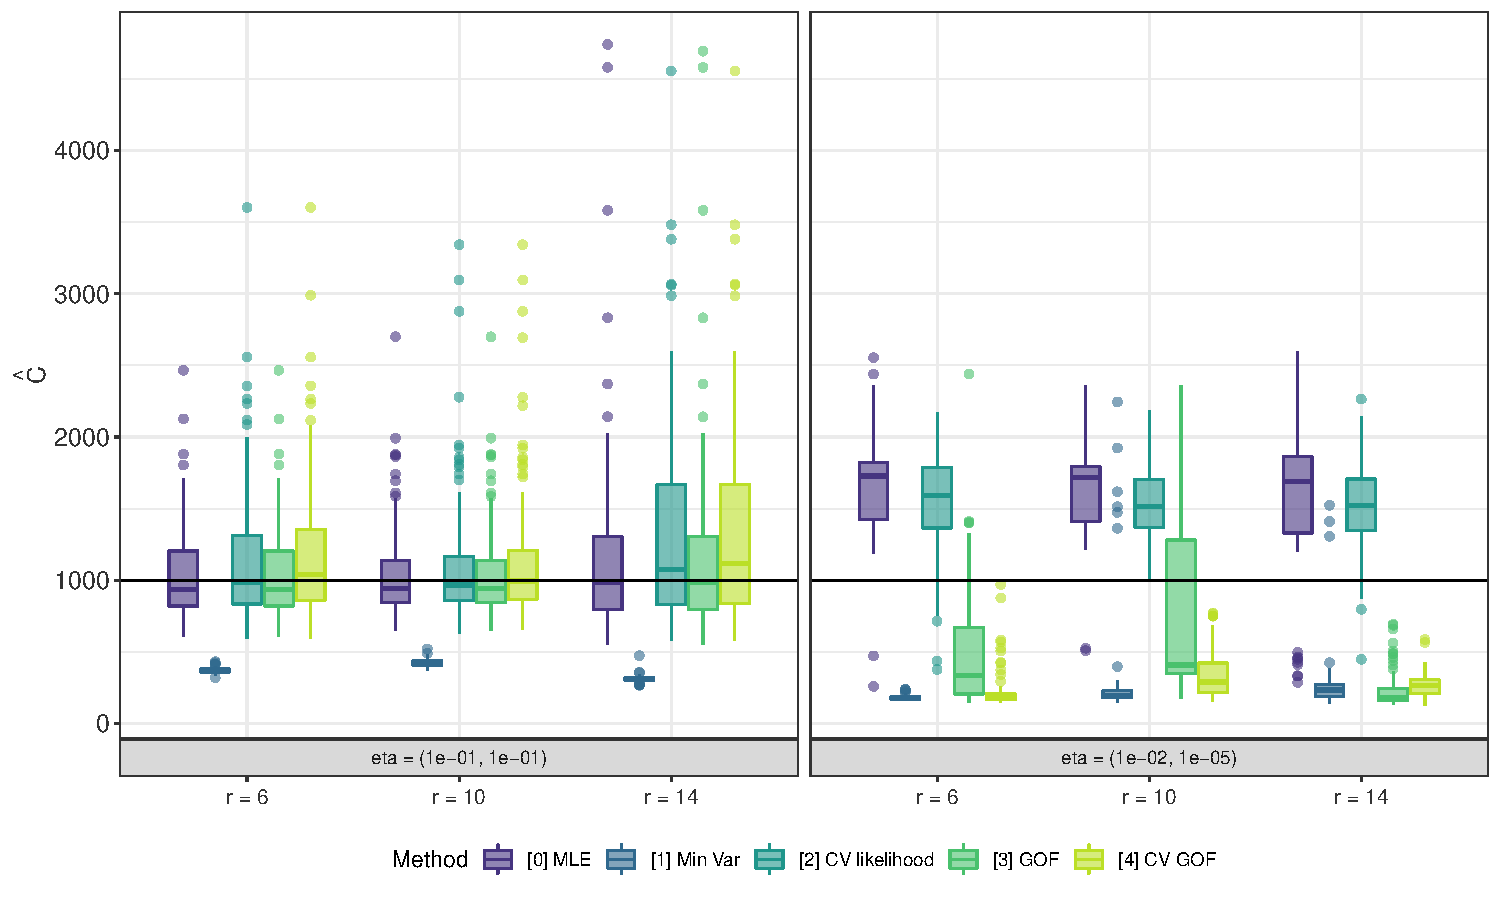
\includegraphics[width=\textwidth]{./images/method_sim_1.pdf}}
\end{figure}

It is clear in Figure \ref{fig:tuning_sim_1} that Method 1 over-penalizes for all parameter choices, as all of the estimates are far below the truth.  We can make sense of this observation based on what we observed in Figure \ref{fig:fixed_lambda}: for very high values of $\lambda$ the estimates have low variance because they are driven down to the observed richness $\max_j c_j$.  However the observed richness has a large negative bias.  Method 1 inherits this large bias as it minimizes variance, so RMSE is not effectively minimized.

Method 2 has the opposite behavior: the estimates tend to be too high, so Method 2 underpenalizes.  This is especially noticeable in $\eta = (10^{-2}, 10^{-5})$, where the Method 0 bias is substantial.  Under this $\eta$ value Method 2 does better than Method 0, but the estimates are almost all too high.

Even for $\eta = (10^{-1}, 10^{-1})$, where the Method 0 bias is smaller, we see that Method 2 has poor performance (Table \ref{tab:tuning_sim_1}).  Recall that in each partition of Method 2 we use only half the data to generate the estimates $\widehat{C}^{T(l)}_{\lambda}$.  As a consequence Method 2 has slightly higher variance when compared with Method 0, as evidenced by the interquartile range in Figure \ref{fig:tuning_sim_1} for $\eta = (10^{-1}, 10^{-1})$.  In conclusion, Method 2 does not seem to be effectively tuning $\lambda$, making the cost of using only half the data to generate estimates especially problematic.

Methods 3 and 4 have different penalization tendencies depending on the $\eta$ and $r$ values of the simulation.  This is a desirable property because we know the optimal $\lambda$ value depends on the structure of the data, and we want a method which can adapt.  In Methods 3 and 4 we generate estimates using the penalized likelihood and evaluate the fit with the goodness of fit metric.  Incorporating two distinct functions may explain why these methods have more adaptable behavior, as opposed to Method 2 which uses likelihood exclusively.

While we find the indications that Method 4 is adaptable to the dataset encouraging, under $\eta = (10^{-1}, 10^{-1})$ the RMSE for Method 4 is 15-75\% greater than for Method 0, while Method 3 is at least as good as Method 0.  Method 3 is adaptive while being simpler, faster and having better performance than Method 4.  Given deficits noted for Method 1 and 2, Method 3 is by far the most promising method based on this simulation.  We propose to conduct a secondary simulation to further challenge Method 3, testing whether it remains superior to Method 0 over a wider range of $\eta$ values.

\subsection{Secondary simulation}
\label{sec:tuning_simulation_2}

\subsubsection{Setup}

In this simulation we will fix $C = 1000$, $r \in \{6, 10, 14\}$ and do 100 simulations for each combination of $\eta, r$ as before.  We let $\eta \in \{ (10^{-1}, 10^{-3}), (10^{-1}, 10^{-5}) \}$ and only consider methods 0 and 3.  To account for the fact that a larger $\lambda$ was optimal for these $\eta$ values (see Table \ref{tab:fixed_lambda_results}) we use $\lambdagrid = \{0,10,20, \dots 140 \}$.

\begin{table}[t]
\tblcaption{RMSE in $\widehat{C}_{[\text{method}]}$.  Simulation parameters are grouped by $\eta$ and $r$, with $C = 1000$ fixed throughout.  Under each $\eta, r$ combination 100 simulations were run.  If Method 3 has better performance than Method 0 is has a \textcolor{blue!50}{blue} background and it is \textbf{bolded}.  This is redundant but consistent with Table \ref{tab:tuning_sim_1}.
\label{tab:tuning_sim_2}}
\centering
\begin{tabular}{|l|c|c|c|c|c|c|}
\cline{2-7}
\multicolumn{1}{c}{} & \multicolumn{3}{|c|}{$\eta = (0.1,0.001)$} & \multicolumn{3}{|c|}{$\eta = (0.1,0.00001)$} \\
\cline{2-7}
\multicolumn{1}{c}{} & \multicolumn{1}{|c|}{$r = 6$} & $r = 10$ & $r = 14$ & $r = 6$ & $r = 10$ & $r = 14$ \\
\hline
Method 0: MLE (no penalization) & \textbf{228} & \textbf{236} & \textbf{188} & \textbf{163} & 426 & 681 \\
\hline
Method 3: Goodness of fit & 260 & 274 & 256 & 183 & \cellcolor{blue!25}{\textbf{175}} & \cellcolor{blue!25}{\textbf{191}} \\
\hline
\end{tabular}
\end{table}

\subsubsection{Results}

In Table \ref{tab:tuning_sim_2} we display the RMSE for both methods and each $\eta, r$ combination.  Method 3 has slightly worse performance on all $r$ values for $\eta = (10^{-1}, 10^{-3})$, with a RMSE which was 14-36\% greater than Method 0.  This $\eta$ generates more rare species so the relatively poor performance of Method 3 is consistent with the results our previous simulation.  In Section \ref{sec:tuning_simulation_1}, Method 3 had greatly improved estimation in data with many abundant species, but the improvements over Method 0 were weaker in datasets that had many rare species.

We also note that Method 3 has 12\% higher RMSE on $r=6, \eta = (10^{-1}, 10^{-5})$, but as $r$ increases Method 3 improves relative to Method 0.  This finding is also consistent with our previous simulation where Method 3 tends to perform better as more data is introduced.

In Figure \ref{fig:tuning_sim_2} we display boxplots of the $C$ estimates over all simulations.  For $\eta = (10^{-2}, 10^{-5})$ we note that $\widehat{C}_{[0]}$ is noticeably inflated on a few simulations.  Referencing Table \ref{tab:eta_intuition} we can recall this $\eta$ choice has the highest proportion of abundant species (while still having some singletons and unobserved species).  Therefore this is a excellent example of a dataset which will cause the instability problem in maximum likelihood estimation we reviewed in Section \ref{sec:literature_review}.  Method 3 succeeds on this $\eta$ primarily by selecting lower estimates on these problematic simulations.

\begin{figure}[t]
\caption{Simulation results for methods 0 and 3 over $\eta = (10^{-1}, 10^{-3})$ and $\eta = (10^{-1}, 10^{-5})$ are shown, with a black line indicating the true value, $C = 1000$.
\label{fig:tuning_sim_2}}
\centering\makebox[\textwidth]{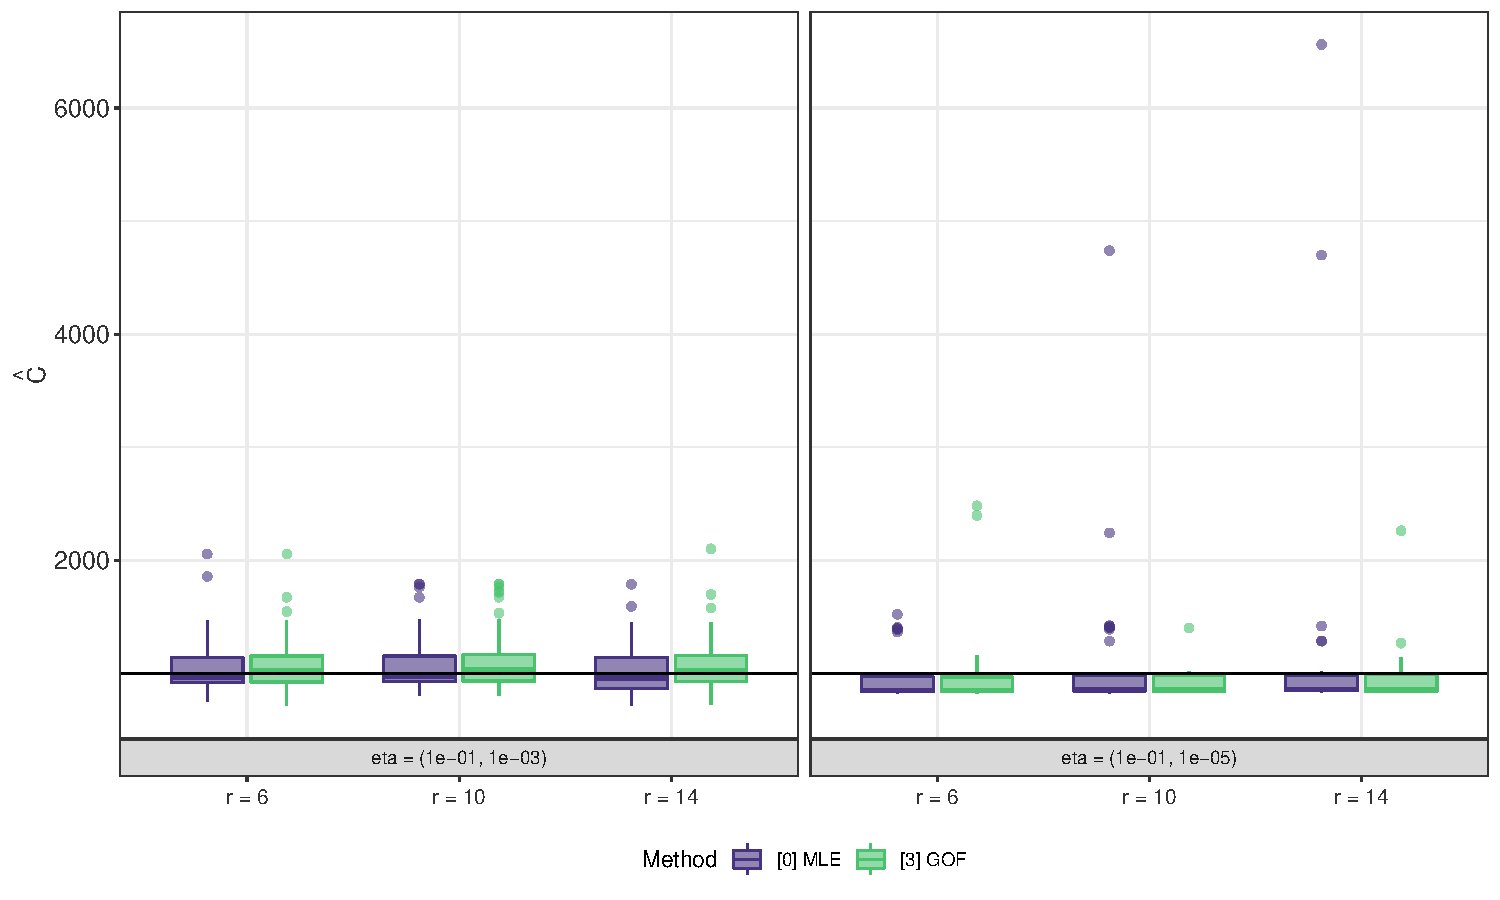
\includegraphics[width=\textwidth]{./images/method_sim_2.pdf}}
\end{figure}

\subsection{Simulation Conclusions}

As a result of these simulations, we conclude that none of the methods (including method 0) are best for all simulation settings.  Method 1 resulted in a strong negative bias no matter which data are being analyzed.  Method 3 had better performance than Method 0 when there are highly abundant species present in the data, which makes Method 0 highly unstable.  When there are many rare species Method 3 is better than methods 1, 2 and 4 but not necessarily Method 0.  Method 3 also improved relative to Method 0 with greater $r$ and appears to better adapt to the data.  Methods 2 and 4 had lower RMSE than Method 0 when highly abundant species exist, but we cannot recommend them over Method 3 due to their inferior performance on data dominated by rare species.

\section{Data Analysis}
\label{sec:data_analysis}

To illustrate the performance of these methods on real data we will use samples collected in consecutive years from Lake Champlain (\citet{tromas_2017}).  We limit our samples to replicates from the summer months and the littoral zone of the lake  (near the shore).  There were 8 replicates meeting these criteria from 2009, 6 replicates from 2010 and 6 from 2011.  The maximum observed richness (most species observed in any replicate that year) was 560 in 2009, 572 in 2010 and 715 in 2011.

The richness estimates from each method are displayed in Table \ref{tab:data_analysis}.  Our estimates from each method are at least 10 times as high as the observed richness, and in some cases they reach the maximum value in our grid search for $C$ (which is 20 times the observed richness).  These extreme estimates suggest that the Gamma-Poisson model which underlies all methods is a poor fit to these data.  In simulations penalization had the intended effect of lowering inflated estimates.  However, we always simulated under a Gamma-Poisson model in simulations.  Using wild data our methods still produce estimates which are suspiciously high.

\begin{table}[t]
\tblcaption{Estimates using a series of three samples from 2009, 2010 and 2011 in the lakes data.  $\widehat{C}_{[\text{method}]}$ is the $C$ estimate obtained using the methods defined in Section \ref{sec:tuning_proposals}, shown for each sample.  The number of replicates in each sample is given by $r$.
\label{tab:data_analysis}}
\centering
\begin{tabular}{|r|r|r|r|}
  \hline
& 2009  & 2010 & 2011 \\
  \hline
$\widehat{C}_{[0]}$ & 11200 & 11440 & 14014 \\
  $\widehat{C}_{[1]}$ & 9645 & 11139 & 12246 \\
  $\widehat{C}_{[2]}$ & 10612 & 11120 & 11946 \\
  $\widehat{C}_{[3]}$ & 11200 & 11440 & 14014 \\
  $\widehat{C}_{[4]}$ & 10744 & 11165 & 10328 \\
   \hline
     $r$ & 8 & 6 & 6 \\
  \hline
\end{tabular}
\end{table}

In Figure \ref{fig:data_analysis} we display the same results visually.  The methods which use partitioning (Methods 1, 2 and 4) consistently produce lower estimates than those which do not (Methods 0 and 3).  This trend was not found in simulations, where the highest estimates came from Method 2 and the lowest from Method 1.  This may suggest that partitioning methods have an advantage on real data which could have greater heterogeneity between replicates than data generated from simple parametric distributions.

\begin{figure}[t]
\caption{A visual display of the results from Table \ref{tab:data_analysis}, $\widehat{C}$ estimates from each method.
\label{fig:data_analysis}}
\centering\makebox[\textwidth]{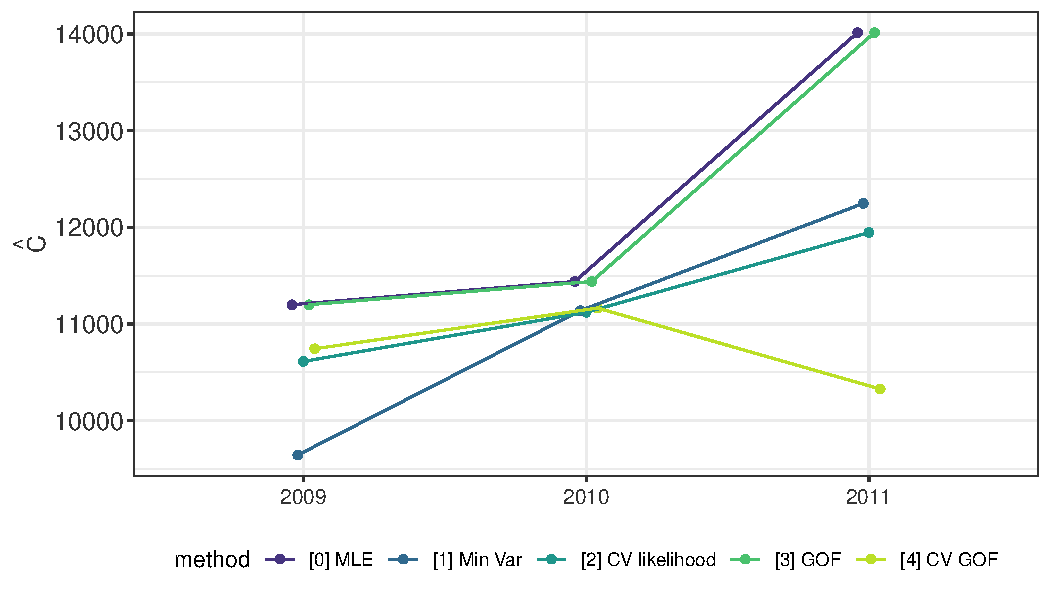
\includegraphics[width=\textwidth]{./images/data_analysis.pdf}}
\end{figure}

\noindent \alex{Next: Modify the discussion to harmonious with what you've written here.}



\section{Discussion}
\label{sec:discussion}

In this paper we have proposed an extension of the penalization in \citet{wang_2005} to data with biological replicates and proposed several methods for tuning the penalization parameter.  This extends the existing body of literature on species richness by demonstrating that penalization is useful in analyzing replicate data.  Our goodness of fit tuning method (Method 3) has better performance than the unpenalized MLE in 8 of the 12 parameter combinations we analyzed.  In this section we note promising directions for future work.{}

Our results from Section \ref{sec:fixed_lambda} hint at a positive correlation between $r$ and the optimal choice of $\lambda$.  We hypothesized that this may be the case and considered other ways of extending the objective function given in Equation \eqref{eq:objective}.  For instance, using $-h(J)\lambda \log p_{\eta}(0)$ where $h(J)$ is $|J|$ or $\sqrt{|J|}$ seemed like plausible extensions, whereas the definition we give uses $h(J) = 1$.  Our investigations revealed that the trend is unfortunately not this simple as $|J|$ becomes large.  A parsimonious extension which accounts for this observed trend would be a valuable modification to our work.

In \citet{wang_2005} the gamma-Poisson model is explicitly considered but their results apply to many other Poisson mixture models.  Our most promising method, Method 3, is also amenable to other modeling choices provided that we have some way to calculate the fitted counts $\widehat{f_k}$.  It would be interesting to explore whether our results hold for a more flexible mixed Poisson distribution, such as the proposal by \citet{norris_1998}.  Flexible models often have better performance under model misspecification, and we simulated under correctly specified models.  Therefore, this variation on  Method 3 would be especially interesting to study under model misspecification.

We intentionally chose a likelihood optimization algorithm which was stable and exhaustive but admittedly slow.  Confirming that our results hold when a faster approach is used would be another valuable extension to our work. We did not derive theoretical standard errors in this paper, and the long computation times precluded the consideration of a bootstrapping approach.  However, if our results hold when a faster likelihood maximization algorithm is used then a standard error procedure could become feasible.

We have been careful to try to create methods which only depend on $\lambdagrid$ being large enough to contain the optimal value, with no change in results if it is too large.  This makes $\lambdagrid$ a more forgiving parameter than fixed $\lambda$ values, but we still need to make a choice to analyze data.  Faster computation times would aid in this problem because we could set a default grid which is generously large, thus alleviating concerns that our results are dependent on our choice.  Additionally, it may be possible to select $\lambdagrid$ for the methods adaptively.  For instance, we could expand the grid until the fixed estimates (e.g. $\widehat{C}_{\lambda}$ in Equation \eqref{eq:c_hat_lambdas_method_3}) have been suppressed to the observed richness.  Choosing $\lambdagrid$ remains a consideration when applying our methods.

Method 3 was our top performer and it is the only tuning method we proposed which can be run without replicates ($r = 1$).  The ever-decreasing cost of high-throughput sequencing suggests biological replicates might be more available in the future.  However, there are currently more projects with a single frequency count table available.  Exploring the use of Method 3 for single frequency count tables is a worthwhile extension of our work for this reason.

\section{Code References}
\label{sec:code}
Our method implementations including our core objective optimization algorithm can be found at \texttt{github.com/statdivlab/rre}.  The code to reproduce our figures and simulations can be found at \texttt{github.com/statdivlab/rre\_sims}.  All code is written in \texttt{R} (\citet{r_project}).


\section*{Acknowledgments}
List of acknowledgements for formalize:

{\it Conflict of Interest}:

\bibliographystyle{biorefs}
\bibliography{refs,amys-papers-library}


\end{document}
